\documentclass[12pt]{article}
\usepackage[margin=2.5cm]{geometry}
\usepackage{enumerate}
\usepackage{amsfonts}
\usepackage{amsmath}
\usepackage{fancyhdr}
\usepackage{amsmath}
\usepackage{amssymb}
\usepackage{amsthm}
\usepackage{mdframed}
\usepackage{graphicx}
\usepackage{subcaption}
\usepackage{adjustbox}
\usepackage{listings}
\usepackage{xcolor}
\usepackage{booktabs}
\usepackage[utf]{kotex}
\usepackage{hyperref}
\usepackage{accents}

\definecolor{codegreen}{rgb}{0,0.6,0}
\definecolor{codegray}{rgb}{0.5,0.5,0.5}
\definecolor{codepurple}{rgb}{0.58,0,0.82}
\definecolor{backcolour}{rgb}{0.95,0.95,0.92}

\lstdefinestyle{mystyle}{
    backgroundcolor=\color{backcolour},
    commentstyle=\color{codegreen},
    keywordstyle=\color{magenta},
    numberstyle=\tiny\color{codegray},
    stringstyle=\color{codepurple},
    basicstyle=\ttfamily\footnotesize,
    breakatwhitespace=false,
    breaklines=true,
    captionpos=b,
    keepspaces=true,
    numbers=left,
    numbersep=5pt,
    showspaces=false,
    showstringspaces=false,
    showtabs=false,
    tabsize=1
}

\lstset{style=mystyle}

\pagestyle{fancy}
\renewcommand{\headrulewidth}{0.4pt}
\lhead{CSC 343}
\rhead{Worksheet 8 Solution}

\begin{document}
\title{CSC343 Worksheet 8 Solution}
\maketitle

\bigskip

\begin{enumerate}[1.]
    \item

    \bigskip

    \begin{enumerate}[a)]
        \item

        \bigskip

        \underline{\textbf{Notes:}}

        \begin{itemize}
            \item Using Call-Level Interface
            \begin{itemize}
                \item Uses host language to connect to and access a database
                \item Replaces embedded SQL
            \end{itemize}
            \item Standard SQL/CLI
            \begin{itemize}
                \item Is database CLI for C
                \item Included in file \textit{sqlcli.h}
                \item Creates deals with four kinds of records

                \bigskip

                \begin{enumerate}[1.]
                    \item Environment handle
                    \begin{itemize}
                        \item Prepares one or more connections to database server
                        \item Is required
                        \item Is allocated using \textbf{SQLHENV}
                        \item Is established via function \textbf{SQLAllocHandle}

                        \begin{center}
                        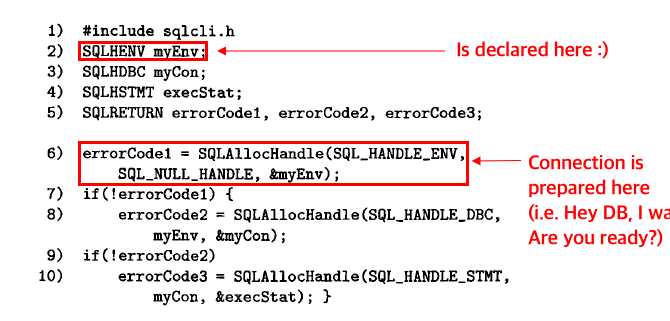
\includegraphics[width=\linewidth]{images/worksheet_8_solution_1.png}
                        \end{center}

                    \end{itemize}
                    \item Connection handle
                    \begin{itemize}
                        \item Conenects application program to database
                        \item Is required
                        \item Is declared after \textbf{SQLHENV}
                        \item Is allocated using \textbf{SQLHDBC}
                        \item Is established via function \textbf{SQLAllocHandle}

                        \begin{center}
                        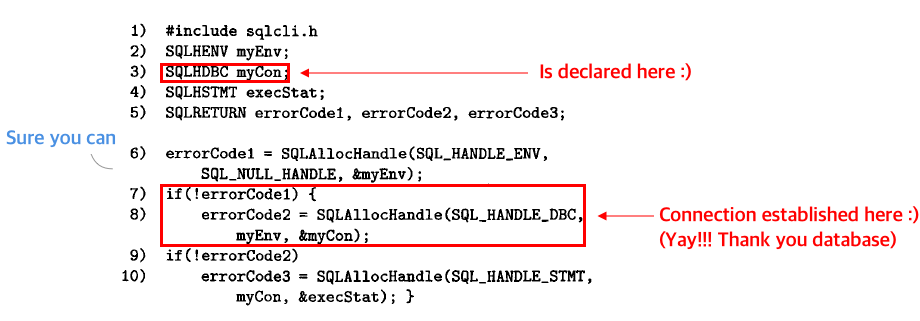
\includegraphics[width=\linewidth]{images/worksheet_8_solution_2.png}
                        \end{center}
                    \end{itemize}
                    \item Statements
                    \begin{itemize}
                        \item Created by application program (the user)
                        \item Can be created as many as needed
                        \item Holds information about a single SQL statement, including cursor
                        \item Can represent different SQL statements at different times
                        \item Is required
                        \item Is declared after \textbf{SQLHDBC}
                        \item Is allocated using \textbf{SQLHSTMT}
                        \item Is sent using the function \textbf{SQLAllocHandle}

                        \begin{center}
                        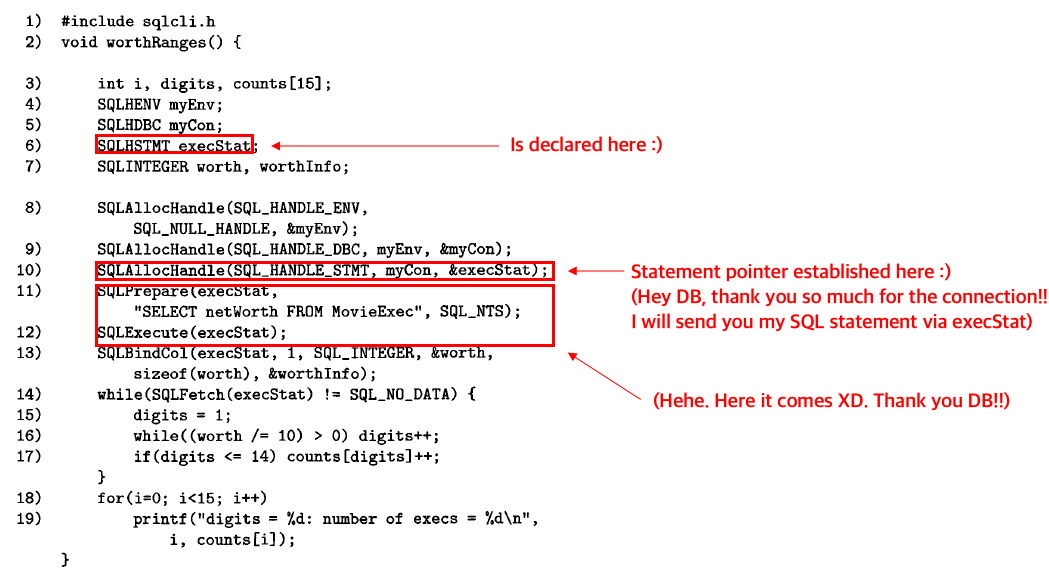
\includegraphics[width=\linewidth]{images/worksheet_8_solution_3.png}
                        \end{center}
                    \end{itemize}
                    \item Descriptions
                    \begin{itemize}
                        \item Holds information about either tuples or parameters
                        \item Each statement has this information implicitly
                    \end{itemize}
                \end{enumerate}
            \end{itemize}
            \item Processing Statements
            \begin{itemize}
                \item is done using \textbf{SQLPrepare} and \textbf{SQLExecute}

                \begin{align}
                    \textbf{SQLPrepare}(sh,st,SQL\_NTS)\\
                    \textbf{SQLExecute}(sh)
                \end{align}

                \item $sh$ is the statement handle created using \textbf{SQLHSTMT}
                \item SQL\_NTS evaluates the length of string in $st$

                \bigskip

                \underline{\textbf{Example:}}

                \bigskip

    \begin{lstlisting}[language=c]
    SQLPrepare(execStat, "SELECT netWorth FROM MovieExec", SQL_NTS);
    SQLExecute(execStat);
    \end{lstlisting}
                \item the function \textbf{SQLExecDirect} combines \textbf{SQLPrepare} and \textbf{SQLExecute}

                \bigskip

                \underline{\textbf{Example 2:}}

                \bigskip

    \begin{lstlisting}[language=c]
    SQLExecDirect(execStat, "SELECT netWorth FROM MovieExec", SQL_NTS);
    \end{lstlisting}
            \end{itemize}
            \item Fetching Data From
            \begin{itemize}
                \item Fetch
                \begin{itemize}
                    \item \textbf{Syntax:} SQLFetch(sh)
                    \item Executes statement in \textbf{SQLPrepare} and \textbf{SQLExecute} and stores result
                    \textbf{SQLBindCol}
                    \item Fetches a row per call
                    \item Returns a value of type \textbf{SQLRETURN}, indicating either success or error
                \end{itemize}
                \item SQLBindCol
                \begin{itemize}
                    \item \textbf{Syntax:} $\text{SQLBindCol}(sh, colNo, colType, pVar, varSize, varInfo)$
                    \begin{itemize}
                        \item \textbf{sh}: the handle of statement
                        \item \textbf{colNo}: the position of column in tuple we obtain
                        \item \textbf{colType}: the SQL data type of variable (i.e. SQL\_INTEGER, SQL\_CHAR)
                        \item \textbf{pVar}: the pointer to variable the value is placed
                        \item \textbf{varSize}: the length in bytes of the value in $pVar$
                        \item \textbf{varInfo}: a pointer to an integer used by SQLBindCol for additional value
                        about the value produced
                    \end{itemize}
                    \item Stores data from \textbf{SQLFetch} to host-language variable
                    \item must be setup before SQLFetch(sh) is run
                \end{itemize}
            \end{itemize}
            \item Passing Parameters to Queries

        \end{itemize}

    \end{enumerate}


\end{enumerate}

\end{document}